\chapter{Validazione} 

In questa fase viene testata la corrispondenza del simulatore con il modello reale. Sono stati effettuati i seguenti controlli:

\begin{itemize}
 \item Saturazione del Front Server: ci sono due concause che portano alla saturazione del Front Server, in primo luogo c'\'e una enorme differenza tra il tasso di servizio di quest'ultimo e quello del Back-End Server che \'e circa 3 volte maggiore; inoltre il numero di utenti che stazionano nel centro Client tende a crescere enormemente e tale comportamento influenza l'andamento di richieste in entrata al Front Server che ne determina la congestione.
 
 \item La coda del Back-End Server risulta essere quasi sempre vuota poich\'e \'e il Front Server che elabora in maniera lenta mentre il tasso di servizio in questo caso \'e di oltre 800 richieste / secondo; questo non permette la creazione di coda e di conseguenza l'utilizzazione \'e molto bassa.
 
 \item Il numero di client \'e notevolmente elevato: questo \'e dovuto all'elevato Think Time sperimentato dagli utenti, circa 7 secondi a client. Considerando il throughput del sistema ed i tassi di servizio dei due serventi \'e immediato notare come il numero dei client attivi contemporaneamente tenda a crescere nel tempo. Tale componente è modellato come un Infinite Server.
 
 \item Nel caso di overload management la percentuale delle connessioni rifiutate e abortite \'e molto alta arrivando a toccare anche l'87\% nel secondo caso, mentre nel primo \'e pi\'u contenuta, con un massimo che si attesta circa attorno al 30\% per poi oscillare in quell'intorno. Questo perch\'e il Front Server rappresenta il collo di bottiglia dell'intero sistema.
\end{itemize}

\section{Modello Analitico}
Al fine di prevedere, in linea di massima, i risultati del simulatore, viene 
elaborato un modello  analitico semplificato per poter studiare il sistema preso 
in esame.
Il sistema implementato presenta numerosi vincoli ed una complessit\'a insita 
nelle specifiche, a tal proposito viene proposto un modello volontariamente e 
lievemente differente dal caso reale, fornendo un limite inferiore delle 
prestazioni e degli indici misurati.

Il sistema esaminato risulta essere interattivo, in quanto avviene uno scambio 
di richieste tra Client e Server, con un comportamento a rete aperta ( le nuove 
sessioni possono entrare nel sistema qualora questo non fosse saturo), a tal 
proposito si \'e deciso di presentare due modelli differenti tra loro, uno a 
rete aperta ed uno a rete chiusa. Questi permettono di descrivere in dettaglio 
la maggior parte degli elementi che costituiscono il sistema stesso.

\section{Modello semplificato a rete aperta}
In questo primo modello si ha una rete aperta di Jackson con un tasso di 
sessioni in
arrivo pari a $\gamma$ . Si \'e deciso cos\'i, per questioni di semplificazione 
del modello, di non
inserire, come componenti, la Priority Queue e il centro di Client, in quanto
risultavano di difficile analisi in un modello di rete aperta come quello di 
Jackson.
\begin{center}	
	\begin{figure}[H]
	\centering
	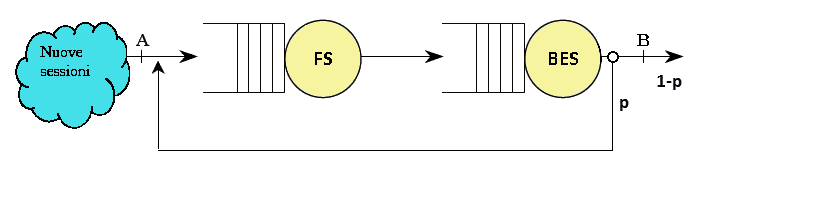
\includegraphics[scale=0.7]{img/reteJackson.png}
	\caption[Modello a rete aperta]{Modello a rete aperta}
	\label{fig:Modello a rete aperta}
	\end{figure}
\end{center}

$\gamma = 35 sessioni/s$

$\vspace{2mm}$

$\begin{cases} 
\lambda_{1} = \gamma + p \lambda_{2} \\ \lambda_{2} = \lambda_{1} \\
\end{cases}$  $\rightarrow$
$\begin{cases} 
\lambda_{1}(1-p) = \gamma \\ \lambda_{2} = \lambda_{1} \\
\end{cases}$ $\rightarrow$
$\begin{cases} 
\lambda_{1} =\frac{ \gamma}{(1- p)} \\ \lambda_{2} =\frac{\lambda_{2}}{(1-p)} \\
\end{cases}$
$\vspace{2mm}$
$\lambda_{1} = \lambda_{2} = \frac{\gamma}{(1-p)} ; p=\frac{19}{20} \rightarrow 
\lambda_{1} = \lambda_{2} = 35\times20 = 700 richieste/s$
$\vspace{2mm}$

$\lambda_{1}\gg\mu_{FS}; \lambda_{2}=\mu_{FS} poichè \mu_{BES}\gg\lambda_{1}$
$\vspace{2mm}$
 Viene quindi calcolato il throughput, ovvero il numero di sessioni che escono 
dal sistema al secondo:
$\vspace{2mm}$

$\lambda_{2} =\frac{\lambda_{2}}{(1-p)}=\frac{\mu_{FS}}{20}\approx\frac{219}{20} 
richieste/s =X_{sessioni}$
$\vspace{2mm}$
$\vspace{2mm}$
$X_{richieste}=X_{sessioni}\times20$
$\vspace{2mm}$
Per quanto concerne l'indice riguardante la percentuale di sessioni rifiutate 
dal sistema, si trova:
$\vspace{2mm}$

$dropped=\frac{\#sessioni accettate}{\#totale arrivi}$ $\rightarrow$ 
$\frac{35-X_{sessioni}}{35} = 1-\frac{2}{7}\approx 0.7$ $\rightarrow$ $\%dropped 
\approx 70\%$

\section{Modello semplificato chiuso}
\begin{center}	
	\begin{figure}[H]
	\centering
	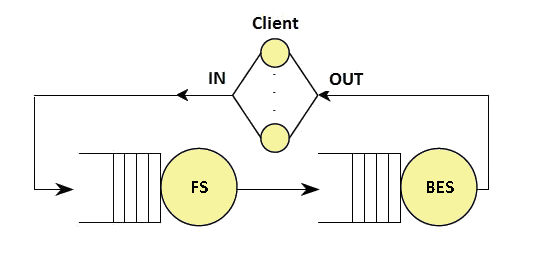
\includegraphics[scale=0.7]{img/retechiusa.png}
	\caption[Modello a rete chiusa]{Modello a rete chiusa}
	\label{fig:Modello a rete aperta}
	\end{figure}
\end{center}

$D_{FS}=0.00456; D_{BES}=0.00117; E[Z]=7s ; N=250$ (in realt\'a il numero 
aumenta costantemente!).
$\vspace{2cm}\hspace{2mm}$
$\vspace{2mm}\hspace{2mm}$ Anche qui si pu\'o calcolare il throughput del 
sistema, come:
$\vspace{2mm}$
$X = min\{\frac{1}{D_{max}},\frac{N}{D+Z}\}= 
min\{\frac{1}{D_{FS}},\frac{250}{D_{FS}+D_{BES}+Z}\}=35.685 richieste/s$.
$\vspace{2mm}$
Da cui si pu\'o ricavare il lower bound per il tempo medio di risposta.
$\vspace{2mm}$
$E[R]\geq max\{D,\frac{N}{X}-E[Z]\}= max 
\{0.00573,\frac{250}{35}-7\}\approx0.0057447$

